We present discuss two Math-in-the-Middle applications that use Jupyter Notebooks for MMT with background knowledge stored in MathHub.info.
The first one is an original OpenDreamKit VRE application focused on computational mathematics as envisioned in the proposal;
the second one arose in the course of the collaboration between WP2 (Micromagnetic VRE for modeling and simulation) and WP6.

\subsection{MitM-Based Formalized Mathematics in MathHub Notebooks}

The MitM approach in  OpenDreamKit uses the MMT language for formalizing mathematical background knowledge and the MMT system for integrating computation tools.
Therefore, Jupyter-MMT notebooks can serve as a unified user interface for MitM systems.

For example, consider the theory at \url{https://gl.mathhub.info/ODK/lmfdb/blob/master/source/schemas/tutorial_example.mmt}, which serves as our standard example for the interaction between MMT and LMFDB (a large database of mathematical objects that was integrated with MMT in previous deliverables of OpenDreamKit).
We can now rewrite it as a notebook.\ednote{@Kai: prepare the notebook, add a link and a screenshot here}

\begin{figure}[ht]\centering
  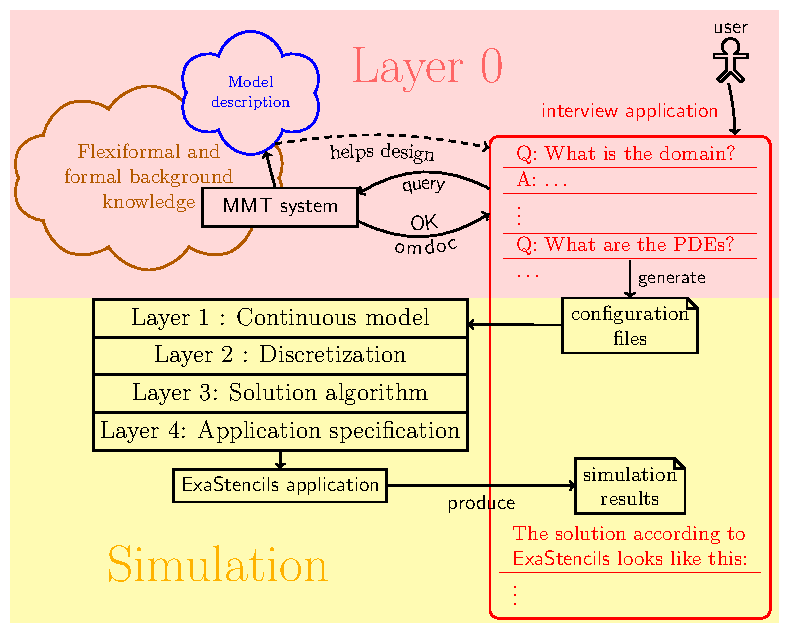
\includegraphics[width=0.6\textwidth]{proto}
  \caption{MoSIS Information Architecture}\label{fig:prototype}
\end{figure}

\subsection{Domain specific applications: MoSIS}

Our second case study addresses a \emph{knowledge gap} that is commonly encountered in computational science and engineering:
To set up a simulation, we need to combine domain knowledge (usually in terms of physical principles), model knowledge (e.g., about suitable partial differential equations) with simulation (i.e., numerics/computing) knowledge.
In pre-VRE practice, this is resolved by intense collaboration between experts, which incurs non-trivial translation and communication overheads.
In OpenDreamKit, we propose an alternate solution based on mathematical knowledge management techniques.
A detailed description was published as \cite{PolKohKoe:kacse18}.

Concretely, we use a Jupyter notebook that has access to an MMT theory graph on MathHub.info.
Figure~\ref{fig:pde-theory} shows this theory graph of background knowledge about mathematical models and partial differential equations.
Our Jupyter/MMT/Mathhub integration enabled building an interview application that hides these mathematical details from the user.  

\begin{figure}[h!p]\centering
  \begin{turn}{-90}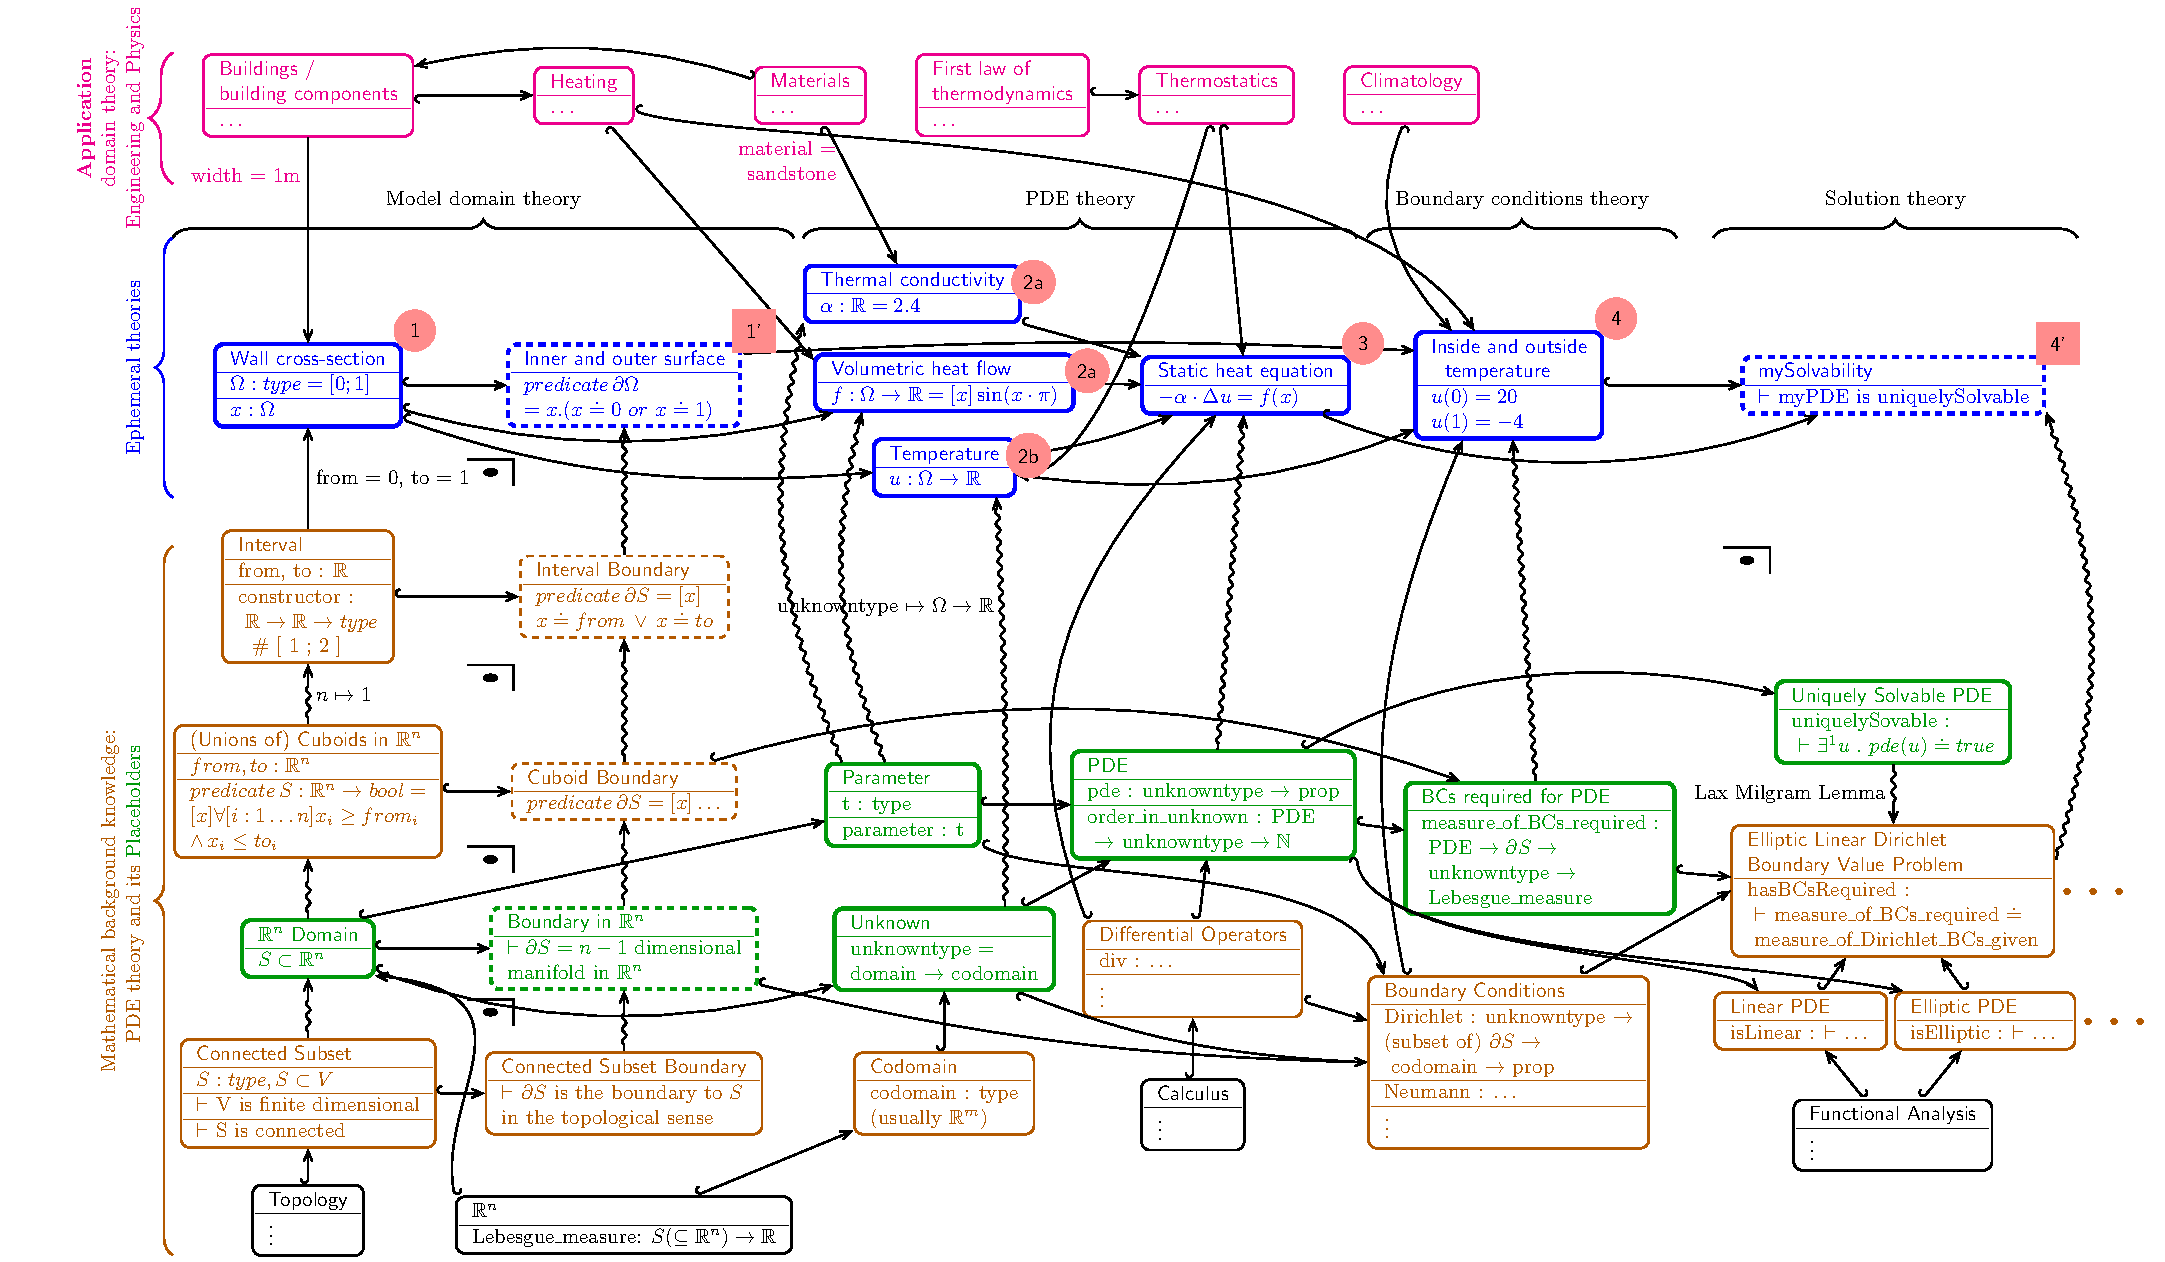
\includegraphics[width=0.95\textheight]{pde-theory}\end{turn}
  \caption{Theory Graph for the MoSIS Case Study}\label{fig:pde-theory}
\end{figure}

Based on this theory graph, we built a targeted knowledge acquisition dialog that supports the formalization of domain knowledge, combines it with simulation knowledge and finally drives a simulation run --- all integrated into a Juypter Notebook.
Figure~\ref{fig:prototype} shows the general architecture:
The left side shows the simulation engine \textsf{ExaStencils} and the MMT system that acts as the theory graph interface.
The right hand side shows the interview --- a Jupyter notebook --- as the active document and how it interacts with the MMT kernel.
The user only sees the notebook.
She answers the knowledge acquisition questions presented by MoSIS until MoSIS can generate a configuration file for ExaStencils.
The latter builds efficient code from it through the ExaSlang layers and computes the results and visualizations, which MoSIS in turn incorporates into the notebook. 
Figure~\ref{fig:int_begin} shows a screenshot of the notebook.

\begin{figure}[ht]
  \fbox{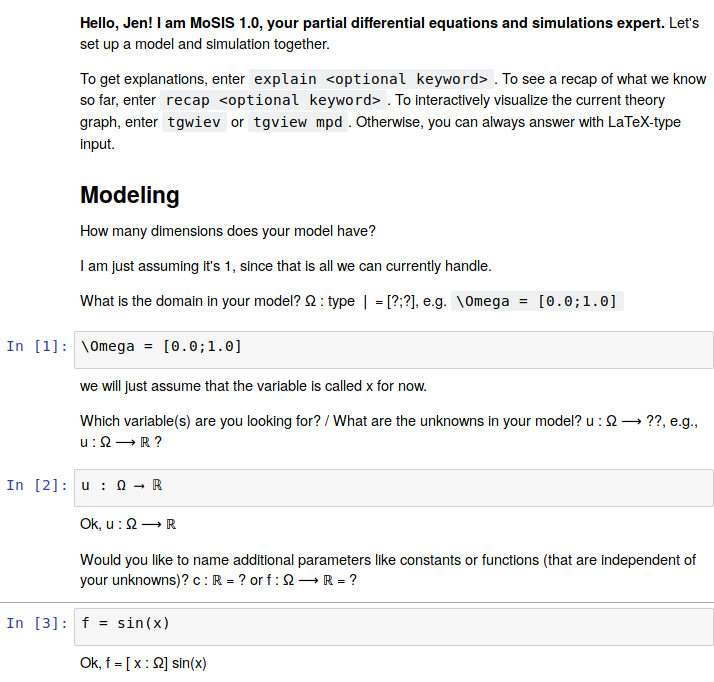
\includegraphics[width=0.8\textwidth]{Screenshot_interview}}
  \caption{Beginning of a Dialogue in MoSIS}\label{fig:int_begin}
\end{figure}

%%% Local Variables:
%%% mode: latex
%%% mode: visual-line
%%% fill-column: 5000
%%% TeX-master: "report"
%%% End:

%  LocalWords:  MitM-Based Formalized formalizing Jupyter-MMT ednote summarize
